\documentclass[twoside]{book}

% Packages required by doxygen
\usepackage{fixltx2e}
\usepackage{calc}
\usepackage{doxygen}
\usepackage[export]{adjustbox} % also loads graphicx
\usepackage{graphicx}
\usepackage[utf8]{inputenc}
\usepackage{makeidx}
\usepackage{multicol}
\usepackage{multirow}
\PassOptionsToPackage{warn}{textcomp}
\usepackage{textcomp}
\usepackage[nointegrals]{wasysym}
\usepackage[table]{xcolor}

% Font selection
\usepackage[T1]{fontenc}
\usepackage[scaled=.90]{helvet}
\usepackage{courier}
\usepackage{amssymb}
\usepackage{sectsty}
\renewcommand{\familydefault}{\sfdefault}
\allsectionsfont{%
  \fontseries{bc}\selectfont%
  \color{darkgray}%
}
\renewcommand{\DoxyLabelFont}{%
  \fontseries{bc}\selectfont%
  \color{darkgray}%
}
\newcommand{\+}{\discretionary{\mbox{\scriptsize$\hookleftarrow$}}{}{}}

% Page & text layout
\usepackage{geometry}
\geometry{%
  a4paper,%
  top=2.5cm,%
  bottom=2.5cm,%
  left=2.5cm,%
  right=2.5cm%
}
\tolerance=750
\hfuzz=15pt
\hbadness=750
\setlength{\emergencystretch}{15pt}
\setlength{\parindent}{0cm}
\setlength{\parskip}{3ex plus 2ex minus 2ex}
\makeatletter
\renewcommand{\paragraph}{%
  \@startsection{paragraph}{4}{0ex}{-1.0ex}{1.0ex}{%
    \normalfont\normalsize\bfseries\SS@parafont%
  }%
}
\renewcommand{\subparagraph}{%
  \@startsection{subparagraph}{5}{0ex}{-1.0ex}{1.0ex}{%
    \normalfont\normalsize\bfseries\SS@subparafont%
  }%
}
\makeatother

% Headers & footers
\usepackage{fancyhdr}
\pagestyle{fancyplain}
\fancyhead[LE]{\fancyplain{}{\bfseries\thepage}}
\fancyhead[CE]{\fancyplain{}{}}
\fancyhead[RE]{\fancyplain{}{\bfseries\leftmark}}
\fancyhead[LO]{\fancyplain{}{\bfseries\rightmark}}
\fancyhead[CO]{\fancyplain{}{}}
\fancyhead[RO]{\fancyplain{}{\bfseries\thepage}}
\fancyfoot[LE]{\fancyplain{}{}}
\fancyfoot[CE]{\fancyplain{}{}}
\fancyfoot[RE]{\fancyplain{}{\bfseries\scriptsize Generated by Doxygen }}
\fancyfoot[LO]{\fancyplain{}{\bfseries\scriptsize Generated by Doxygen }}
\fancyfoot[CO]{\fancyplain{}{}}
\fancyfoot[RO]{\fancyplain{}{}}
\renewcommand{\footrulewidth}{0.4pt}
\renewcommand{\chaptermark}[1]{%
  \markboth{#1}{}%
}
\renewcommand{\sectionmark}[1]{%
  \markright{\thesection\ #1}%
}

% Indices & bibliography
\usepackage{natbib}
\usepackage[titles]{tocloft}
\setcounter{tocdepth}{3}
\setcounter{secnumdepth}{5}
\makeindex

% Hyperlinks (required, but should be loaded last)
\usepackage{ifpdf}
\ifpdf
  \usepackage[pdftex,pagebackref=true]{hyperref}
\else
  \usepackage[ps2pdf,pagebackref=true]{hyperref}
\fi
\hypersetup{%
  colorlinks=true,%
  linkcolor=blue,%
  citecolor=blue,%
  unicode%
}

% Custom commands
\newcommand{\clearemptydoublepage}{%
  \newpage{\pagestyle{empty}\cleardoublepage}%
}

\usepackage{caption}
\captionsetup{labelsep=space,justification=centering,font={bf},singlelinecheck=off,skip=4pt,position=top}

%===== C O N T E N T S =====

\begin{document}

% Titlepage & ToC
\hypersetup{pageanchor=false,
             bookmarksnumbered=true,
             pdfencoding=unicode
            }
\pagenumbering{alph}
\begin{titlepage}
\vspace*{7cm}
\begin{center}%
{\Large team-\/algoriths-\/oops }\\
\vspace*{1cm}
{\large Generated by Doxygen 1.8.13}\\
\end{center}
\end{titlepage}
\clearemptydoublepage
\pagenumbering{roman}
\tableofcontents
\clearemptydoublepage
\pagenumbering{arabic}
\hypersetup{pageanchor=true}

%--- Begin generated contents ---
\chapter{Namespace Index}
\section{Namespace List}
Here is a list of all documented namespaces with brief descriptions\+:\begin{DoxyCompactList}
\item\contentsline{section}{\hyperlink{namespacelab_1_1forest}{lab\+::forest} \\*Namespace that contains implementations of all trees }{\pageref{namespacelab_1_1forest}}{}
\item\contentsline{section}{\hyperlink{namespacelab_1_1forest_1_1detail}{lab\+::forest\+::detail} \\*Set of functions to work with binary tree nodes }{\pageref{namespacelab_1_1forest_1_1detail}}{}
\end{DoxyCompactList}

\chapter{Hierarchical Index}
\section{Class Hierarchy}
This inheritance list is sorted roughly, but not completely, alphabetically\+:\begin{DoxyCompactList}
\item \contentsline{section}{lab\+:\+:forest\+:\+:Any\+Tree$<$ Value\+Type, Supported\+Comparators $>$}{\pageref{classlab_1_1forest_1_1AnyTree}}{}
\item \contentsline{section}{lab\+:\+:forest\+:\+:detail\+:\+:B\+S\+T\+Base$<$ T, Compare, Derived\+Tree $>$}{\pageref{classlab_1_1forest_1_1detail_1_1BSTBase}}{}
\item \contentsline{section}{lab\+:\+:forest\+:\+:detail\+:\+:B\+S\+T\+Base$<$ T, Compare, Red\+Black\+Tree$<$ T, Compare $>$ $>$}{\pageref{classlab_1_1forest_1_1detail_1_1BSTBase}}{}
\begin{DoxyCompactList}
\item \contentsline{section}{lab\+:\+:forest\+:\+:Red\+Black\+Tree$<$ T, Compare $>$}{\pageref{classlab_1_1forest_1_1RedBlackTree}}{}
\end{DoxyCompactList}
\item \contentsline{section}{lab\+:\+:forest\+:\+:detail\+:\+:B\+S\+T\+Base$<$ T, Compare, Splay\+Tree$<$ T, Compare $>$ $>$}{\pageref{classlab_1_1forest_1_1detail_1_1BSTBase}}{}
\begin{DoxyCompactList}
\item \contentsline{section}{lab\+:\+:forest\+:\+:Splay\+Tree$<$ T, Compare $>$}{\pageref{classlab_1_1forest_1_1SplayTree}}{}
\end{DoxyCompactList}
\item \contentsline{section}{lab\+:\+:forest\+:\+:detail\+:\+:B\+S\+T\+Iterator$<$ Tree $>$}{\pageref{classlab_1_1forest_1_1detail_1_1BSTIterator}}{}
\item \contentsline{section}{lab\+:\+:forest\+:\+:detail\+:\+:Node$<$ Tree $>$}{\pageref{structlab_1_1forest_1_1detail_1_1Node}}{}
\item \contentsline{section}{lab\+:\+:forest\+:\+:detail\+:\+:Node$<$ Derived\+Tree $>$}{\pageref{structlab_1_1forest_1_1detail_1_1Node}}{}
\item \contentsline{section}{lab\+:\+:forest\+:\+:detail\+:\+:Node$<$ Red\+Black\+Tree$<$ T, Compare $>$ $>$}{\pageref{structlab_1_1forest_1_1detail_1_1Node}}{}
\item \contentsline{section}{lab\+:\+:forest\+:\+:detail\+:\+:Node$<$ Splay\+Tree$<$ T, Compare $>$ $>$}{\pageref{structlab_1_1forest_1_1detail_1_1Node}}{}
\item \contentsline{section}{lab\+:\+:Tree\+Database}{\pageref{classlab_1_1TreeDatabase}}{}
\item \contentsline{section}{lab\+:\+:forest\+:\+:Undoable\+Tree$<$ Tree $>$}{\pageref{classlab_1_1forest_1_1UndoableTree}}{}
\end{DoxyCompactList}

\chapter{Class Index}
\section{Class List}
Here are the classes, structs, unions and interfaces with brief descriptions\+:\begin{DoxyCompactList}
\item\contentsline{section}{\hyperlink{classlab_1_1forest_1_1AnyTree}{lab\+::forest\+::\+Any\+Tree$<$ Value\+Type, Supported\+Comparators $>$} \\*Class that can hold object of any tree and gives interface to work with it }{\pageref{classlab_1_1forest_1_1AnyTree}}{}
\item\contentsline{section}{\hyperlink{classlab_1_1forest_1_1detail_1_1BSTBase}{lab\+::forest\+::detail\+::\+B\+S\+T\+Base$<$ T, Compare, Derived\+Tree $>$} \\*Abstract base class for binary search tree implementations using C\+R\+TP }{\pageref{classlab_1_1forest_1_1detail_1_1BSTBase}}{}
\item\contentsline{section}{\hyperlink{classlab_1_1forest_1_1detail_1_1BSTIterator}{lab\+::forest\+::detail\+::\+B\+S\+T\+Iterator$<$ Tree $>$} \\*Tree Iterator for binary search tree with node that has pointer on parent node }{\pageref{classlab_1_1forest_1_1detail_1_1BSTIterator}}{}
\item\contentsline{section}{\hyperlink{structlab_1_1forest_1_1detail_1_1Node}{lab\+::forest\+::detail\+::\+Node$<$ Tree $>$} \\*Tree node class, use class template specialization for your tree implementations }{\pageref{structlab_1_1forest_1_1detail_1_1Node}}{}
\item\contentsline{section}{\hyperlink{classlab_1_1forest_1_1RedBlackTree}{lab\+::forest\+::\+Red\+Black\+Tree$<$ T, Compare $>$} \\*Red-\/\+Black Tree implementation T -\/ type of value stored in tree, Compare -\/ comparison function class for elements in tree }{\pageref{classlab_1_1forest_1_1RedBlackTree}}{}
\item\contentsline{section}{\hyperlink{classlab_1_1forest_1_1SplayTree}{lab\+::forest\+::\+Splay\+Tree$<$ T, Compare $>$} \\*Splay Tree implementation T -\/ type of value stored in tree, Compare -\/ comparison function class for elements in tree }{\pageref{classlab_1_1forest_1_1SplayTree}}{}
\item\contentsline{section}{\hyperlink{classlab_1_1TreeDatabase}{lab\+::\+Tree\+Database} \\*Singleton class represention S\+Q\+Lite-\/based database for tree (can be any container) }{\pageref{classlab_1_1TreeDatabase}}{}
\item\contentsline{section}{\hyperlink{classlab_1_1forest_1_1UndoableTree}{lab\+::forest\+::\+Undoable\+Tree$<$ Tree $>$} \\*Class that expand Tree functionality by undo and redo operations }{\pageref{classlab_1_1forest_1_1UndoableTree}}{}
\end{DoxyCompactList}

\chapter{Namespace Documentation}
\hypertarget{namespacelab_1_1forest}{}\section{lab\+:\+:forest Namespace Reference}
\label{namespacelab_1_1forest}\index{lab\+::forest@{lab\+::forest}}


Namespace that contains implementations of all trees.  


\subsection*{Namespaces}
\begin{DoxyCompactItemize}
\item 
 \hyperlink{namespacelab_1_1forest_1_1detail}{detail}
\begin{DoxyCompactList}\small\item\em Set of functions to work with binary tree nodes. \end{DoxyCompactList}\end{DoxyCompactItemize}
\subsection*{Classes}
\begin{DoxyCompactItemize}
\item 
class \hyperlink{classlab_1_1forest_1_1AnyTree}{Any\+Tree}
\begin{DoxyCompactList}\small\item\em Class that can hold object of any tree and gives interface to work with it. \end{DoxyCompactList}\item 
class \hyperlink{classlab_1_1forest_1_1RedBlackTree}{Red\+Black\+Tree}
\begin{DoxyCompactList}\small\item\em Red-\/\+Black Tree implementation T -\/ type of value stored in tree, Compare -\/ comparison function class for elements in tree. \end{DoxyCompactList}\item 
class \hyperlink{classlab_1_1forest_1_1SplayTree}{Splay\+Tree}
\begin{DoxyCompactList}\small\item\em Splay Tree implementation T -\/ type of value stored in tree, Compare -\/ comparison function class for elements in tree. \end{DoxyCompactList}\item 
class \hyperlink{classlab_1_1forest_1_1UndoableTree}{Undoable\+Tree}
\begin{DoxyCompactList}\small\item\em Class that expand Tree functionality by undo and redo operations. \end{DoxyCompactList}\end{DoxyCompactItemize}
\subsection*{Functions}
\begin{DoxyCompactItemize}
\item 
\mbox{\Hypertarget{namespacelab_1_1forest_ae2a6f2027fb35965ce66d355d7a6ccad}\label{namespacelab_1_1forest_ae2a6f2027fb35965ce66d355d7a6ccad}} 
{\footnotesize template$<$typename Tree $>$ }\\{\bfseries Any\+Tree} (const Tree \&\+\_\+tree) -\/$>$ \hyperlink{classlab_1_1forest_1_1AnyTree}{Any\+Tree}$<$ typename Tree\+::value\+\_\+type $>$
\end{DoxyCompactItemize}


\subsection{Detailed Description}
Namespace that contains implementations of all trees. 
\hypertarget{namespacelab_1_1forest_1_1detail}{}\section{lab\+:\+:forest\+:\+:detail Namespace Reference}
\label{namespacelab_1_1forest_1_1detail}\index{lab\+::forest\+::detail@{lab\+::forest\+::detail}}


Set of functions to work with binary tree nodes.  


\subsection*{Classes}
\begin{DoxyCompactItemize}
\item 
class \hyperlink{classlab_1_1forest_1_1detail_1_1BSTBase}{B\+S\+T\+Base}
\begin{DoxyCompactList}\small\item\em Abstract base class for binary search tree implementations using C\+R\+TP. \end{DoxyCompactList}\item 
class \hyperlink{classlab_1_1forest_1_1detail_1_1BSTIterator}{B\+S\+T\+Iterator}
\begin{DoxyCompactList}\small\item\em Tree Iterator for binary search tree with node that has pointer on parent node. \end{DoxyCompactList}\item 
struct \hyperlink{structlab_1_1forest_1_1detail_1_1Node}{Node}
\begin{DoxyCompactList}\small\item\em Tree node class, use class template specialization for your tree implementations. \end{DoxyCompactList}\end{DoxyCompactItemize}
\subsection*{Functions}
\begin{DoxyCompactItemize}
\item 
\mbox{\Hypertarget{namespacelab_1_1forest_1_1detail_ad6c94d5f86fe169609f866b00bb12ca4}\label{namespacelab_1_1forest_1_1detail_ad6c94d5f86fe169609f866b00bb12ca4}} 
{\footnotesize template$<$typename Tree $>$ }\\{\bfseries B\+S\+T\+Iterator} (\hyperlink{structlab_1_1forest_1_1detail_1_1Node}{Node}$<$ Tree $>$ $\ast$root) -\/$>$ \hyperlink{classlab_1_1forest_1_1detail_1_1BSTIterator}{B\+S\+T\+Iterator}$<$ Tree $>$
\item 
\mbox{\Hypertarget{namespacelab_1_1forest_1_1detail_afb98b9a3926409e631bb25e421435948}\label{namespacelab_1_1forest_1_1detail_afb98b9a3926409e631bb25e421435948}} 
{\footnotesize template$<$typename Tree , typename T , typename Compare $>$ }\\auto \hyperlink{namespacelab_1_1forest_1_1detail_afb98b9a3926409e631bb25e421435948}{find} (\hyperlink{structlab_1_1forest_1_1detail_1_1Node}{Node}$<$ Tree $>$ $\ast$node, const T \&elem, const Compare \&comp) noexcept -\/$>$ \hyperlink{structlab_1_1forest_1_1detail_1_1Node}{Node}$<$ Tree $>$ $\ast$
\begin{DoxyCompactList}\small\item\em Returns node with key elem in subtree node. \end{DoxyCompactList}\item 
\mbox{\Hypertarget{namespacelab_1_1forest_1_1detail_a8232fa106684cfa32c642cdc74588020}\label{namespacelab_1_1forest_1_1detail_a8232fa106684cfa32c642cdc74588020}} 
{\footnotesize template$<$typename Tree $>$ }\\bool {\bfseries is\+Left\+Son} (\hyperlink{structlab_1_1forest_1_1detail_1_1Node}{Node}$<$ Tree $>$ $\ast$node) noexcept
\item 
\mbox{\Hypertarget{namespacelab_1_1forest_1_1detail_a4d272afcedeaeab259efea52775a1e64}\label{namespacelab_1_1forest_1_1detail_a4d272afcedeaeab259efea52775a1e64}} 
{\footnotesize template$<$typename Tree $>$ }\\bool {\bfseries is\+Right\+Son} (\hyperlink{structlab_1_1forest_1_1detail_1_1Node}{Node}$<$ Tree $>$ $\ast$node) noexcept
\item 
{\footnotesize template$<$typename Tree $>$ }\\auto \hyperlink{namespacelab_1_1forest_1_1detail_a56c6d104e669b3ae029cf7ddbd79e72f}{min} (\hyperlink{structlab_1_1forest_1_1detail_1_1Node}{Node}$<$ Tree $>$ $\ast$node) noexcept -\/$>$ \hyperlink{structlab_1_1forest_1_1detail_1_1Node}{Node}$<$ Tree $>$ $\ast$
\item 
{\footnotesize template$<$typename Tree $>$ }\\auto \hyperlink{namespacelab_1_1forest_1_1detail_a1b854c05579f96cde71983fa181a4f5f}{max} (\hyperlink{structlab_1_1forest_1_1detail_1_1Node}{Node}$<$ Tree $>$ $\ast$node) noexcept -\/$>$ \hyperlink{structlab_1_1forest_1_1detail_1_1Node}{Node}$<$ Tree $>$ $\ast$
\item 
\mbox{\Hypertarget{namespacelab_1_1forest_1_1detail_a21acd0d04e9a7cae68b7fe60da6d1948}\label{namespacelab_1_1forest_1_1detail_a21acd0d04e9a7cae68b7fe60da6d1948}} 
{\footnotesize template$<$typename Tree $>$ }\\void \hyperlink{namespacelab_1_1forest_1_1detail_a21acd0d04e9a7cae68b7fe60da6d1948}{copy\+Node\+Data} (\hyperlink{structlab_1_1forest_1_1detail_1_1Node}{Node}$<$ Tree $>$ $\ast$to\+Copy, \hyperlink{structlab_1_1forest_1_1detail_1_1Node}{Node}$<$ Tree $>$ $\ast$to\+Paste)
\begin{DoxyCompactList}\small\item\em Copy field of to\+Copy node to to\+Paste node, but without fields-\/pointers. \end{DoxyCompactList}\item 
{\footnotesize template$<$typename Tree $>$ }\\auto \hyperlink{namespacelab_1_1forest_1_1detail_a1268b660bcac79b1fb63758a157cba64}{clone} (\hyperlink{structlab_1_1forest_1_1detail_1_1Node}{Node}$<$ Tree $>$ $\ast$node, \hyperlink{structlab_1_1forest_1_1detail_1_1Node}{Node}$<$ Tree $>$ $\ast$parent\+Node=nullptr) -\/$>$ \hyperlink{structlab_1_1forest_1_1detail_1_1Node}{Node}$<$ Tree $>$ $\ast$
\item 
\mbox{\Hypertarget{namespacelab_1_1forest_1_1detail_a1036d00410feb4a2aa3683ec5831f071}\label{namespacelab_1_1forest_1_1detail_a1036d00410feb4a2aa3683ec5831f071}} 
{\footnotesize template$<$typename Tree , typename Compare $>$ }\\auto \hyperlink{namespacelab_1_1forest_1_1detail_a1036d00410feb4a2aa3683ec5831f071}{insert} (\hyperlink{structlab_1_1forest_1_1detail_1_1Node}{Node}$<$ Tree $>$ $\ast$node, \hyperlink{structlab_1_1forest_1_1detail_1_1Node}{Node}$<$ Tree $>$ $\ast$to\+\_\+insert, const Compare \&comp) -\/$>$ \hyperlink{structlab_1_1forest_1_1detail_1_1Node}{detail\+::\+Node}$<$ Tree $>$ $\ast$
\begin{DoxyCompactList}\small\item\em Simple insertion in B\+ST node without parent info, non-\/recursive approach. \end{DoxyCompactList}\item 
\mbox{\Hypertarget{namespacelab_1_1forest_1_1detail_a55dbdf697d2acd430c4631fe9f521844}\label{namespacelab_1_1forest_1_1detail_a55dbdf697d2acd430c4631fe9f521844}} 
{\footnotesize template$<$typename Tree , typename Compare $>$ }\\auto \hyperlink{namespacelab_1_1forest_1_1detail_a55dbdf697d2acd430c4631fe9f521844}{insert\+With\+Parent} (\hyperlink{structlab_1_1forest_1_1detail_1_1Node}{Node}$<$ Tree $>$ $\ast$node, \hyperlink{structlab_1_1forest_1_1detail_1_1Node}{Node}$<$ Tree $>$ $\ast$to\+\_\+insert, const Compare \&comp) -\/$>$ \hyperlink{structlab_1_1forest_1_1detail_1_1Node}{Node}$<$ Tree $>$ $\ast$
\begin{DoxyCompactList}\small\item\em Simple insertion in B\+ST node with parent info, non-\/recursive approach. \end{DoxyCompactList}\item 
\mbox{\Hypertarget{namespacelab_1_1forest_1_1detail_ab9ab28094d14db3c2db76078fc30e7d1}\label{namespacelab_1_1forest_1_1detail_ab9ab28094d14db3c2db76078fc30e7d1}} 
{\footnotesize template$<$typename Tree $>$ }\\void \hyperlink{namespacelab_1_1forest_1_1detail_ab9ab28094d14db3c2db76078fc30e7d1}{set} (\hyperlink{structlab_1_1forest_1_1detail_1_1Node}{Node}$<$ Tree $>$ $\ast$\&var, \hyperlink{structlab_1_1forest_1_1detail_1_1Node}{Node}$<$ Tree $>$ $\ast$value, \hyperlink{structlab_1_1forest_1_1detail_1_1Node}{Node}$<$ Tree $>$ $\ast$new\+\_\+parent=nullptr)
\begin{DoxyCompactList}\small\item\em Assign var to value, setting var\textquotesingle{}s parent new\+\_\+parent. \end{DoxyCompactList}\item 
\mbox{\Hypertarget{namespacelab_1_1forest_1_1detail_a14b2355c9f8bcb8e2e625e19635ad723}\label{namespacelab_1_1forest_1_1detail_a14b2355c9f8bcb8e2e625e19635ad723}} 
{\footnotesize template$<$typename Tree $>$ }\\void \hyperlink{namespacelab_1_1forest_1_1detail_a14b2355c9f8bcb8e2e625e19635ad723}{make\+Ordered\+Sequence} (\hyperlink{structlab_1_1forest_1_1detail_1_1Node}{Node}$<$ Tree $>$ $\ast$node, std\+::vector$<$ \hyperlink{structlab_1_1forest_1_1detail_1_1Node}{Node}$<$ Tree $>$ $\ast$$>$ \&nodes)
\begin{DoxyCompactList}\small\item\em Fills std\+::vector of all nodes of subtree \textquotesingle{}node\textquotesingle{} in increasing order. \end{DoxyCompactList}\item 
{\footnotesize template$<$typename Tree $>$ }\\void \hyperlink{namespacelab_1_1forest_1_1detail_aaf762170657e2de7273548d147d2d913}{right\+Rotate} (\hyperlink{structlab_1_1forest_1_1detail_1_1Node}{Node}$<$ Tree $>$ $\ast$node)
\item 
{\footnotesize template$<$typename Tree $>$ }\\void \hyperlink{namespacelab_1_1forest_1_1detail_a726d38cf7417fa78151bd039ebb75acc}{left\+Rotate} (\hyperlink{structlab_1_1forest_1_1detail_1_1Node}{Node}$<$ Tree $>$ $\ast$node)
\item 
{\footnotesize template$<$typename Tree $>$ }\\auto \hyperlink{namespacelab_1_1forest_1_1detail_a77eddeb28a75cfb0360c39c0146b1827}{sibling} (\hyperlink{structlab_1_1forest_1_1detail_1_1Node}{Node}$<$ Tree $>$ $\ast$node) -\/$>$ \hyperlink{structlab_1_1forest_1_1detail_1_1Node}{Node}$<$ Tree $>$ $\ast$
\item 
\mbox{\Hypertarget{namespacelab_1_1forest_1_1detail_a034971d1100329df601f507135123322}\label{namespacelab_1_1forest_1_1detail_a034971d1100329df601f507135123322}} 
{\footnotesize template$<$typename Tree $>$ }\\void {\bfseries swap\+Data} (\hyperlink{structlab_1_1forest_1_1detail_1_1Node}{Node}$<$ Tree $>$ $\ast$first\+Node, \hyperlink{structlab_1_1forest_1_1detail_1_1Node}{Node}$<$ Tree $>$ $\ast$second\+Node)
\item 
\mbox{\Hypertarget{namespacelab_1_1forest_1_1detail_a159f4606df5b6cd691d20409af15fb0d}\label{namespacelab_1_1forest_1_1detail_a159f4606df5b6cd691d20409af15fb0d}} 
{\footnotesize template$<$typename Tree $>$ }\\void \hyperlink{namespacelab_1_1forest_1_1detail_a159f4606df5b6cd691d20409af15fb0d}{erase\+Sub\+Tree} (\hyperlink{structlab_1_1forest_1_1detail_1_1Node}{Node}$<$ Tree $>$ $\ast$to\+Delete)
\begin{DoxyCompactList}\small\item\em Recurrsively erase whole subtree strating from to\+Delete node. \end{DoxyCompactList}\item 
{\footnotesize template$<$typename Tree $>$ }\\auto \hyperlink{namespacelab_1_1forest_1_1detail_a708d9e4ef9e2c273fe36235b092dbd25}{find\+Replacement} (\hyperlink{structlab_1_1forest_1_1detail_1_1Node}{Node}$<$ Tree $>$ $\ast$node) -\/$>$ \hyperlink{structlab_1_1forest_1_1detail_1_1Node}{Node}$<$ Tree $>$ $\ast$
\begin{DoxyCompactList}\small\item\em Find the closest node which can be put in place of given node. \end{DoxyCompactList}\end{DoxyCompactItemize}


\subsection{Detailed Description}
Set of functions to work with binary tree nodes. 

\subsection{Function Documentation}
\mbox{\Hypertarget{namespacelab_1_1forest_1_1detail_a1268b660bcac79b1fb63758a157cba64}\label{namespacelab_1_1forest_1_1detail_a1268b660bcac79b1fb63758a157cba64}} 
\index{lab\+::forest\+::detail@{lab\+::forest\+::detail}!clone@{clone}}
\index{clone@{clone}!lab\+::forest\+::detail@{lab\+::forest\+::detail}}
\subsubsection{\texorpdfstring{clone()}{clone()}}
{\footnotesize\ttfamily template$<$typename Tree $>$ \\
auto lab\+::forest\+::detail\+::clone (\begin{DoxyParamCaption}\item[{\hyperlink{structlab_1_1forest_1_1detail_1_1Node}{Node}$<$ Tree $>$ $\ast$}]{node,  }\item[{\hyperlink{structlab_1_1forest_1_1detail_1_1Node}{Node}$<$ Tree $>$ $\ast$}]{parent\+Node = {\ttfamily nullptr} }\end{DoxyParamCaption}) -\/$>$ \hyperlink{structlab_1_1forest_1_1detail_1_1Node}{Node}$<$Tree$>$$\ast$ }

\begin{DoxyReturn}{Returns}
Deep copy of node 
\end{DoxyReturn}
\mbox{\Hypertarget{namespacelab_1_1forest_1_1detail_a708d9e4ef9e2c273fe36235b092dbd25}\label{namespacelab_1_1forest_1_1detail_a708d9e4ef9e2c273fe36235b092dbd25}} 
\index{lab\+::forest\+::detail@{lab\+::forest\+::detail}!find\+Replacement@{find\+Replacement}}
\index{find\+Replacement@{find\+Replacement}!lab\+::forest\+::detail@{lab\+::forest\+::detail}}
\subsubsection{\texorpdfstring{find\+Replacement()}{findReplacement()}}
{\footnotesize\ttfamily template$<$typename Tree $>$ \\
auto lab\+::forest\+::detail\+::find\+Replacement (\begin{DoxyParamCaption}\item[{\hyperlink{structlab_1_1forest_1_1detail_1_1Node}{Node}$<$ Tree $>$ $\ast$}]{node }\end{DoxyParamCaption}) -\/$>$ \hyperlink{structlab_1_1forest_1_1detail_1_1Node}{Node}$<$Tree$>$$\ast$ }



Find the closest node which can be put in place of given node. 


\begin{DoxyParams}{Parameters}
{\em node} & \hyperlink{structlab_1_1forest_1_1detail_1_1Node}{Node} for which we should find replacement node \\
\hline
\end{DoxyParams}
\begin{DoxyReturn}{Returns}
\hyperlink{structlab_1_1forest_1_1detail_1_1Node}{Node} that should replace given node 
\end{DoxyReturn}
\mbox{\Hypertarget{namespacelab_1_1forest_1_1detail_a726d38cf7417fa78151bd039ebb75acc}\label{namespacelab_1_1forest_1_1detail_a726d38cf7417fa78151bd039ebb75acc}} 
\index{lab\+::forest\+::detail@{lab\+::forest\+::detail}!left\+Rotate@{left\+Rotate}}
\index{left\+Rotate@{left\+Rotate}!lab\+::forest\+::detail@{lab\+::forest\+::detail}}
\subsubsection{\texorpdfstring{left\+Rotate()}{leftRotate()}}
{\footnotesize\ttfamily template$<$typename Tree $>$ \\
void lab\+::forest\+::detail\+::left\+Rotate (\begin{DoxyParamCaption}\item[{\hyperlink{structlab_1_1forest_1_1detail_1_1Node}{Node}$<$ Tree $>$ $\ast$}]{node }\end{DoxyParamCaption})}


\begin{DoxyParams}{Parameters}
{\em node} & right child of current parent after rotation becomes parent \\
\hline
\end{DoxyParams}
\mbox{\Hypertarget{namespacelab_1_1forest_1_1detail_a1b854c05579f96cde71983fa181a4f5f}\label{namespacelab_1_1forest_1_1detail_a1b854c05579f96cde71983fa181a4f5f}} 
\index{lab\+::forest\+::detail@{lab\+::forest\+::detail}!max@{max}}
\index{max@{max}!lab\+::forest\+::detail@{lab\+::forest\+::detail}}
\subsubsection{\texorpdfstring{max()}{max()}}
{\footnotesize\ttfamily template$<$typename Tree $>$ \\
auto lab\+::forest\+::detail\+::max (\begin{DoxyParamCaption}\item[{\hyperlink{structlab_1_1forest_1_1detail_1_1Node}{Node}$<$ Tree $>$ $\ast$}]{node }\end{DoxyParamCaption}) -\/$>$ \hyperlink{structlab_1_1forest_1_1detail_1_1Node}{Node}$<$Tree$>$$\ast$ \hspace{0.3cm}{\ttfamily [noexcept]}}

\begin{DoxyReturn}{Returns}
\hyperlink{structlab_1_1forest_1_1detail_1_1Node}{Node} with max element in subtree 
\end{DoxyReturn}
\mbox{\Hypertarget{namespacelab_1_1forest_1_1detail_a56c6d104e669b3ae029cf7ddbd79e72f}\label{namespacelab_1_1forest_1_1detail_a56c6d104e669b3ae029cf7ddbd79e72f}} 
\index{lab\+::forest\+::detail@{lab\+::forest\+::detail}!min@{min}}
\index{min@{min}!lab\+::forest\+::detail@{lab\+::forest\+::detail}}
\subsubsection{\texorpdfstring{min()}{min()}}
{\footnotesize\ttfamily template$<$typename Tree $>$ \\
auto lab\+::forest\+::detail\+::min (\begin{DoxyParamCaption}\item[{\hyperlink{structlab_1_1forest_1_1detail_1_1Node}{Node}$<$ Tree $>$ $\ast$}]{node }\end{DoxyParamCaption}) -\/$>$ \hyperlink{structlab_1_1forest_1_1detail_1_1Node}{Node}$<$Tree$>$$\ast$ \hspace{0.3cm}{\ttfamily [noexcept]}}

\begin{DoxyReturn}{Returns}
\hyperlink{structlab_1_1forest_1_1detail_1_1Node}{Node} with min element in subtree 
\end{DoxyReturn}
\mbox{\Hypertarget{namespacelab_1_1forest_1_1detail_aaf762170657e2de7273548d147d2d913}\label{namespacelab_1_1forest_1_1detail_aaf762170657e2de7273548d147d2d913}} 
\index{lab\+::forest\+::detail@{lab\+::forest\+::detail}!right\+Rotate@{right\+Rotate}}
\index{right\+Rotate@{right\+Rotate}!lab\+::forest\+::detail@{lab\+::forest\+::detail}}
\subsubsection{\texorpdfstring{right\+Rotate()}{rightRotate()}}
{\footnotesize\ttfamily template$<$typename Tree $>$ \\
void lab\+::forest\+::detail\+::right\+Rotate (\begin{DoxyParamCaption}\item[{\hyperlink{structlab_1_1forest_1_1detail_1_1Node}{Node}$<$ Tree $>$ $\ast$}]{node }\end{DoxyParamCaption})}


\begin{DoxyParams}{Parameters}
{\em node} & left child of current parent after rotation becomes parent \\
\hline
\end{DoxyParams}
\mbox{\Hypertarget{namespacelab_1_1forest_1_1detail_a77eddeb28a75cfb0360c39c0146b1827}\label{namespacelab_1_1forest_1_1detail_a77eddeb28a75cfb0360c39c0146b1827}} 
\index{lab\+::forest\+::detail@{lab\+::forest\+::detail}!sibling@{sibling}}
\index{sibling@{sibling}!lab\+::forest\+::detail@{lab\+::forest\+::detail}}
\subsubsection{\texorpdfstring{sibling()}{sibling()}}
{\footnotesize\ttfamily template$<$typename Tree $>$ \\
auto lab\+::forest\+::detail\+::sibling (\begin{DoxyParamCaption}\item[{\hyperlink{structlab_1_1forest_1_1detail_1_1Node}{Node}$<$ Tree $>$ $\ast$}]{node }\end{DoxyParamCaption}) -\/$>$ \hyperlink{structlab_1_1forest_1_1detail_1_1Node}{Node}$<$Tree$>$$\ast$ }

\begin{DoxyReturn}{Returns}
Another child of node parent and nullptr if there is no parent 
\end{DoxyReturn}

\chapter{Class Documentation}
\hypertarget{classlab_1_1forest_1_1AnyTree}{}\section{lab\+:\+:forest\+:\+:Any\+Tree$<$ Value\+Type, Supported\+Comparators $>$ Class Template Reference}
\label{classlab_1_1forest_1_1AnyTree}\index{lab\+::forest\+::\+Any\+Tree$<$ Value\+Type, Supported\+Comparators $>$@{lab\+::forest\+::\+Any\+Tree$<$ Value\+Type, Supported\+Comparators $>$}}


Class that can hold object of any tree and gives interface to work with it.  




{\ttfamily \#include $<$Any\+Tree.\+hpp$>$}



\subsection{Detailed Description}
\subsubsection*{template$<$typename Value\+Type, typename Supported\+Comparators = Supported\+Comparators$<$std\+::less$<$$>$$>$$>$\newline
class lab\+::forest\+::\+Any\+Tree$<$ Value\+Type, Supported\+Comparators $>$}

Class that can hold object of any tree and gives interface to work with it. 

The documentation for this class was generated from the following file\+:\begin{DoxyCompactItemize}
\item 
include/Any\+Tree.\+hpp\end{DoxyCompactItemize}

\hypertarget{classlab_1_1forest_1_1detail_1_1BSTBase}{}\section{lab\+:\+:forest\+:\+:detail\+:\+:B\+S\+T\+Base$<$ T, Compare, Derived\+Tree $>$ Class Template Reference}
\label{classlab_1_1forest_1_1detail_1_1BSTBase}\index{lab\+::forest\+::detail\+::\+B\+S\+T\+Base$<$ T, Compare, Derived\+Tree $>$@{lab\+::forest\+::detail\+::\+B\+S\+T\+Base$<$ T, Compare, Derived\+Tree $>$}}


Abstract base class for binary search tree implementations using C\+R\+TP.  




{\ttfamily \#include $<$B\+S\+T\+Base.\+hpp$>$}



Collaboration diagram for lab\+:\+:forest\+:\+:detail\+:\+:B\+S\+T\+Base$<$ T, Compare, Derived\+Tree $>$\+:
\nopagebreak
\begin{figure}[H]
\begin{center}
\leavevmode
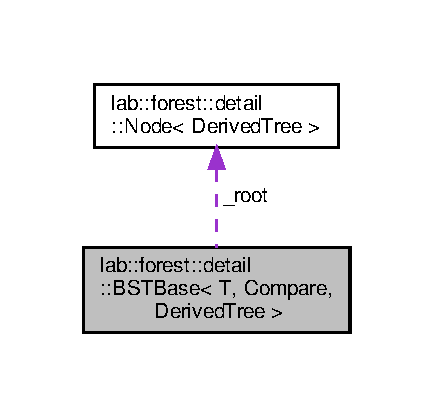
\includegraphics[width=208pt]{classlab_1_1forest_1_1detail_1_1BSTBase__coll__graph}
\end{center}
\end{figure}
\subsection*{Public Types}
\begin{DoxyCompactItemize}
\item 
\mbox{\Hypertarget{classlab_1_1forest_1_1detail_1_1BSTBase_ab100bb39d2607700286a707c40dcac11}\label{classlab_1_1forest_1_1detail_1_1BSTBase_ab100bb39d2607700286a707c40dcac11}} 
using {\bfseries value\+\_\+type} = T
\item 
\mbox{\Hypertarget{classlab_1_1forest_1_1detail_1_1BSTBase_a6a6e409005b5922c1f9217d699cc965e}\label{classlab_1_1forest_1_1detail_1_1BSTBase_a6a6e409005b5922c1f9217d699cc965e}} 
using {\bfseries iterator} = \hyperlink{classlab_1_1forest_1_1detail_1_1BSTIterator}{B\+S\+T\+Iterator}$<$ Derived\+Tree $>$
\end{DoxyCompactItemize}
\subsection*{Public Member Functions}
\begin{DoxyCompactItemize}
\item 
\hyperlink{classlab_1_1forest_1_1detail_1_1BSTIterator}{iterator} \hyperlink{classlab_1_1forest_1_1detail_1_1BSTBase_aac3bd1152a3754526dcc429c30f74ffb}{search} (const T \&key) noexcept
\item 
\mbox{\Hypertarget{classlab_1_1forest_1_1detail_1_1BSTBase_a7b0c4d929e60a583e4fefc88fe0979ac}\label{classlab_1_1forest_1_1detail_1_1BSTBase_a7b0c4d929e60a583e4fefc88fe0979ac}} 
void \hyperlink{classlab_1_1forest_1_1detail_1_1BSTBase_a7b0c4d929e60a583e4fefc88fe0979ac}{insert} (const T \&key)
\begin{DoxyCompactList}\small\item\em Inserts key to tree. \end{DoxyCompactList}\item 
\mbox{\Hypertarget{classlab_1_1forest_1_1detail_1_1BSTBase_ab5b55f3b275ce011aee2a8ad4bd18fb3}\label{classlab_1_1forest_1_1detail_1_1BSTBase_ab5b55f3b275ce011aee2a8ad4bd18fb3}} 
void \hyperlink{classlab_1_1forest_1_1detail_1_1BSTBase_ab5b55f3b275ce011aee2a8ad4bd18fb3}{erase} (const T \&key)
\begin{DoxyCompactList}\small\item\em Erase element with this key from tree. \end{DoxyCompactList}\item 
\hyperlink{classlab_1_1forest_1_1detail_1_1BSTIterator}{iterator} \hyperlink{classlab_1_1forest_1_1detail_1_1BSTBase_aee57d4461130971ad187ea41bc8e4e74}{begin} () const noexcept
\item 
\hyperlink{classlab_1_1forest_1_1detail_1_1BSTIterator}{iterator} \hyperlink{classlab_1_1forest_1_1detail_1_1BSTBase_ad2ea364cc61d5581a861d1aab3734129}{end} () const noexcept
\item 
\mbox{\Hypertarget{classlab_1_1forest_1_1detail_1_1BSTBase_a518f44b8f05298ea36f382ad9c558ce1}\label{classlab_1_1forest_1_1detail_1_1BSTBase_a518f44b8f05298ea36f382ad9c558ce1}} 
{\bfseries B\+S\+T\+Base} (const \hyperlink{classlab_1_1forest_1_1detail_1_1BSTBase}{B\+S\+T\+Base} \&other)
\item 
\mbox{\Hypertarget{classlab_1_1forest_1_1detail_1_1BSTBase_a7f56344789a083f9b0efd5c6190c4af6}\label{classlab_1_1forest_1_1detail_1_1BSTBase_a7f56344789a083f9b0efd5c6190c4af6}} 
{\bfseries B\+S\+T\+Base} (\hyperlink{classlab_1_1forest_1_1detail_1_1BSTBase}{B\+S\+T\+Base} \&\&other) noexcept
\item 
\mbox{\Hypertarget{classlab_1_1forest_1_1detail_1_1BSTBase_ac56cd574b026e98ddb2aeca457d5d898}\label{classlab_1_1forest_1_1detail_1_1BSTBase_ac56cd574b026e98ddb2aeca457d5d898}} 
\hyperlink{classlab_1_1forest_1_1detail_1_1BSTBase}{B\+S\+T\+Base} \& {\bfseries operator=} (Derived\+Tree other) noexcept
\item 
\mbox{\Hypertarget{classlab_1_1forest_1_1detail_1_1BSTBase_a7bb7f10ef641e7057949c00cf8cc812b}\label{classlab_1_1forest_1_1detail_1_1BSTBase_a7bb7f10ef641e7057949c00cf8cc812b}} 
\hyperlink{classlab_1_1forest_1_1detail_1_1BSTBase}{B\+S\+T\+Base} \& {\bfseries operator=} (const \hyperlink{classlab_1_1forest_1_1detail_1_1BSTBase}{B\+S\+T\+Base} \&other) noexcept=default
\item 
\mbox{\Hypertarget{classlab_1_1forest_1_1detail_1_1BSTBase_ac578b147c53ab2f0a18a15756d94ac76}\label{classlab_1_1forest_1_1detail_1_1BSTBase_ac578b147c53ab2f0a18a15756d94ac76}} 
\hyperlink{classlab_1_1forest_1_1detail_1_1BSTBase}{B\+S\+T\+Base} \& {\bfseries operator=} (\hyperlink{classlab_1_1forest_1_1detail_1_1BSTBase}{B\+S\+T\+Base} \&\&other) noexcept=default
\item 
\mbox{\Hypertarget{classlab_1_1forest_1_1detail_1_1BSTBase_aaf5f2af7dd8862c7e2181eec6a767bfa}\label{classlab_1_1forest_1_1detail_1_1BSTBase_aaf5f2af7dd8862c7e2181eec6a767bfa}} 
bool {\bfseries operator==} (const Derived\+Tree \&other) const noexcept
\item 
\mbox{\Hypertarget{classlab_1_1forest_1_1detail_1_1BSTBase_a48843ab8cae5c4246bddc895f634de53}\label{classlab_1_1forest_1_1detail_1_1BSTBase_a48843ab8cae5c4246bddc895f634de53}} 
bool {\bfseries operator!=} (const Derived\+Tree \&other) const noexcept
\item 
auto \hyperlink{classlab_1_1forest_1_1detail_1_1BSTBase_a26625c36d62d907106f61a33f793777b}{size} () const noexcept -\/$>$ std\+::size\+\_\+t
\item 
auto \hyperlink{classlab_1_1forest_1_1detail_1_1BSTBase_a8986f7a9fd8ef965740f0fd1acd71dd3}{compare\+Func} () const noexcept -\/$>$ Compare
\end{DoxyCompactItemize}
\subsection*{Protected Member Functions}
\begin{DoxyCompactItemize}
\item 
\mbox{\Hypertarget{classlab_1_1forest_1_1detail_1_1BSTBase_af77ccebd03c9e2fb80b462b0e231f1ae}\label{classlab_1_1forest_1_1detail_1_1BSTBase_af77ccebd03c9e2fb80b462b0e231f1ae}} 
{\bfseries B\+S\+T\+Base} (const Compare \&comp=Compare\{\})
\item 
\mbox{\Hypertarget{classlab_1_1forest_1_1detail_1_1BSTBase_a9691e34ec314b525967888ad09e8717a}\label{classlab_1_1forest_1_1detail_1_1BSTBase_a9691e34ec314b525967888ad09e8717a}} 
void {\bfseries simple\+Insert} (\hyperlink{structlab_1_1forest_1_1detail_1_1Node}{lab\+::forest\+::detail\+::\+Node}$<$ Derived\+Tree $>$ $\ast$to\+Insert)
\end{DoxyCompactItemize}
\subsection*{Protected Attributes}
\begin{DoxyCompactItemize}
\item 
\mbox{\Hypertarget{classlab_1_1forest_1_1detail_1_1BSTBase_af2d79489ceab33ecfa6a6c90df7bd12f}\label{classlab_1_1forest_1_1detail_1_1BSTBase_af2d79489ceab33ecfa6a6c90df7bd12f}} 
std\+::size\+\_\+t {\bfseries \+\_\+size} = 0
\item 
\mbox{\Hypertarget{classlab_1_1forest_1_1detail_1_1BSTBase_ac956fd4baf6a5a055f2eebea66aebafb}\label{classlab_1_1forest_1_1detail_1_1BSTBase_ac956fd4baf6a5a055f2eebea66aebafb}} 
Compare {\bfseries \+\_\+comp} = Compare\{\}
\item 
\mbox{\Hypertarget{classlab_1_1forest_1_1detail_1_1BSTBase_acf863c0027cb1d90ac099917f5a988d4}\label{classlab_1_1forest_1_1detail_1_1BSTBase_acf863c0027cb1d90ac099917f5a988d4}} 
\hyperlink{structlab_1_1forest_1_1detail_1_1Node}{lab\+::forest\+::detail\+::\+Node}$<$ Derived\+Tree $>$ $\ast$ {\bfseries \+\_\+root} = nullptr
\end{DoxyCompactItemize}
\subsection*{Friends}
\begin{DoxyCompactItemize}
\item 
\mbox{\Hypertarget{classlab_1_1forest_1_1detail_1_1BSTBase_ad7b611157b688b63c666ce6caecd6e0b}\label{classlab_1_1forest_1_1detail_1_1BSTBase_ad7b611157b688b63c666ce6caecd6e0b}} 
void \hyperlink{classlab_1_1forest_1_1detail_1_1BSTBase_ad7b611157b688b63c666ce6caecd6e0b}{swap} (\hyperlink{classlab_1_1forest_1_1detail_1_1BSTBase}{B\+S\+T\+Base} \&lhs, \hyperlink{classlab_1_1forest_1_1detail_1_1BSTBase}{B\+S\+T\+Base} \&rhs) noexcept
\begin{DoxyCompactList}\small\item\em Swaps contents of trees. \end{DoxyCompactList}\end{DoxyCompactItemize}


\subsection{Detailed Description}
\subsubsection*{template$<$typename T, typename Compare, typename Derived\+Tree$>$\newline
class lab\+::forest\+::detail\+::\+B\+S\+T\+Base$<$ T, Compare, Derived\+Tree $>$}

Abstract base class for binary search tree implementations using C\+R\+TP. 

Provides B\+ST iterator, representing elements in increasing order and \hyperlink{classlab_1_1forest_1_1detail_1_1BSTBase_aee57d4461130971ad187ea41bc8e4e74}{begin()}, \hyperlink{classlab_1_1forest_1_1detail_1_1BSTBase_ad2ea364cc61d5581a861d1aab3734129}{end()} methods. Provides search and size methods, copy and move constuctors, copy and move assigment operators, and swap function. Requires insert\+Impl(const T\& key) and erase\+Impl(const T\& key) methods in derived class. Implementation details like root and size are protected. 

\subsection{Member Function Documentation}
\mbox{\Hypertarget{classlab_1_1forest_1_1detail_1_1BSTBase_aee57d4461130971ad187ea41bc8e4e74}\label{classlab_1_1forest_1_1detail_1_1BSTBase_aee57d4461130971ad187ea41bc8e4e74}} 
\index{lab\+::forest\+::detail\+::\+B\+S\+T\+Base@{lab\+::forest\+::detail\+::\+B\+S\+T\+Base}!begin@{begin}}
\index{begin@{begin}!lab\+::forest\+::detail\+::\+B\+S\+T\+Base@{lab\+::forest\+::detail\+::\+B\+S\+T\+Base}}
\subsubsection{\texorpdfstring{begin()}{begin()}}
{\footnotesize\ttfamily template$<$typename T, typename Compare, typename Derived\+Tree$>$ \\
\hyperlink{classlab_1_1forest_1_1detail_1_1BSTIterator}{iterator} \hyperlink{classlab_1_1forest_1_1detail_1_1BSTBase}{lab\+::forest\+::detail\+::\+B\+S\+T\+Base}$<$ T, Compare, Derived\+Tree $>$\+::begin (\begin{DoxyParamCaption}{ }\end{DoxyParamCaption}) const\hspace{0.3cm}{\ttfamily [noexcept]}}

\begin{DoxyReturn}{Returns}
Iterator pointed to the min element in tree 
\end{DoxyReturn}
\mbox{\Hypertarget{classlab_1_1forest_1_1detail_1_1BSTBase_a8986f7a9fd8ef965740f0fd1acd71dd3}\label{classlab_1_1forest_1_1detail_1_1BSTBase_a8986f7a9fd8ef965740f0fd1acd71dd3}} 
\index{lab\+::forest\+::detail\+::\+B\+S\+T\+Base@{lab\+::forest\+::detail\+::\+B\+S\+T\+Base}!compare\+Func@{compare\+Func}}
\index{compare\+Func@{compare\+Func}!lab\+::forest\+::detail\+::\+B\+S\+T\+Base@{lab\+::forest\+::detail\+::\+B\+S\+T\+Base}}
\subsubsection{\texorpdfstring{compare\+Func()}{compareFunc()}}
{\footnotesize\ttfamily template$<$typename T, typename Compare, typename Derived\+Tree$>$ \\
auto \hyperlink{classlab_1_1forest_1_1detail_1_1BSTBase}{lab\+::forest\+::detail\+::\+B\+S\+T\+Base}$<$ T, Compare, Derived\+Tree $>$\+::compare\+Func (\begin{DoxyParamCaption}{ }\end{DoxyParamCaption}) const -\/$>$  Compare\hspace{0.3cm}{\ttfamily [noexcept]}}

\begin{DoxyReturn}{Returns}
Function that sets order in tree, default -\/ std\+::less\{\} 
\end{DoxyReturn}
\mbox{\Hypertarget{classlab_1_1forest_1_1detail_1_1BSTBase_ad2ea364cc61d5581a861d1aab3734129}\label{classlab_1_1forest_1_1detail_1_1BSTBase_ad2ea364cc61d5581a861d1aab3734129}} 
\index{lab\+::forest\+::detail\+::\+B\+S\+T\+Base@{lab\+::forest\+::detail\+::\+B\+S\+T\+Base}!end@{end}}
\index{end@{end}!lab\+::forest\+::detail\+::\+B\+S\+T\+Base@{lab\+::forest\+::detail\+::\+B\+S\+T\+Base}}
\subsubsection{\texorpdfstring{end()}{end()}}
{\footnotesize\ttfamily template$<$typename T, typename Compare, typename Derived\+Tree$>$ \\
\hyperlink{classlab_1_1forest_1_1detail_1_1BSTIterator}{iterator} \hyperlink{classlab_1_1forest_1_1detail_1_1BSTBase}{lab\+::forest\+::detail\+::\+B\+S\+T\+Base}$<$ T, Compare, Derived\+Tree $>$\+::end (\begin{DoxyParamCaption}{ }\end{DoxyParamCaption}) const\hspace{0.3cm}{\ttfamily [noexcept]}}

\begin{DoxyReturn}{Returns}
Iterator pointed to the element after last in tree 
\end{DoxyReturn}
\begin{DoxyWarning}{Warning}
Use only to check if element is in tree, derefencing causes exception 
\end{DoxyWarning}
\mbox{\Hypertarget{classlab_1_1forest_1_1detail_1_1BSTBase_aac3bd1152a3754526dcc429c30f74ffb}\label{classlab_1_1forest_1_1detail_1_1BSTBase_aac3bd1152a3754526dcc429c30f74ffb}} 
\index{lab\+::forest\+::detail\+::\+B\+S\+T\+Base@{lab\+::forest\+::detail\+::\+B\+S\+T\+Base}!search@{search}}
\index{search@{search}!lab\+::forest\+::detail\+::\+B\+S\+T\+Base@{lab\+::forest\+::detail\+::\+B\+S\+T\+Base}}
\subsubsection{\texorpdfstring{search()}{search()}}
{\footnotesize\ttfamily template$<$typename T, typename Compare, typename Derived\+Tree$>$ \\
\hyperlink{classlab_1_1forest_1_1detail_1_1BSTIterator}{iterator} \hyperlink{classlab_1_1forest_1_1detail_1_1BSTBase}{lab\+::forest\+::detail\+::\+B\+S\+T\+Base}$<$ T, Compare, Derived\+Tree $>$\+::search (\begin{DoxyParamCaption}\item[{const T \&}]{key }\end{DoxyParamCaption})\hspace{0.3cm}{\ttfamily [noexcept]}}

\begin{DoxyReturn}{Returns}
Iterator to key in tree, if not found -\/ \hyperlink{classlab_1_1forest_1_1detail_1_1BSTBase_ad2ea364cc61d5581a861d1aab3734129}{end()} 
\end{DoxyReturn}
\mbox{\Hypertarget{classlab_1_1forest_1_1detail_1_1BSTBase_a26625c36d62d907106f61a33f793777b}\label{classlab_1_1forest_1_1detail_1_1BSTBase_a26625c36d62d907106f61a33f793777b}} 
\index{lab\+::forest\+::detail\+::\+B\+S\+T\+Base@{lab\+::forest\+::detail\+::\+B\+S\+T\+Base}!size@{size}}
\index{size@{size}!lab\+::forest\+::detail\+::\+B\+S\+T\+Base@{lab\+::forest\+::detail\+::\+B\+S\+T\+Base}}
\subsubsection{\texorpdfstring{size()}{size()}}
{\footnotesize\ttfamily template$<$typename T, typename Compare, typename Derived\+Tree$>$ \\
auto \hyperlink{classlab_1_1forest_1_1detail_1_1BSTBase}{lab\+::forest\+::detail\+::\+B\+S\+T\+Base}$<$ T, Compare, Derived\+Tree $>$\+::size (\begin{DoxyParamCaption}{ }\end{DoxyParamCaption}) const -\/$>$  std\+::size\+\_\+t\hspace{0.3cm}{\ttfamily [noexcept]}}

\begin{DoxyReturn}{Returns}
Amount of elements in tree 
\end{DoxyReturn}


The documentation for this class was generated from the following file\+:\begin{DoxyCompactItemize}
\item 
src/B\+S\+T\+Base.\+hpp\end{DoxyCompactItemize}

\hypertarget{classlab_1_1forest_1_1detail_1_1BSTIterator}{}\section{lab\+:\+:forest\+:\+:detail\+:\+:B\+S\+T\+Iterator$<$ Tree $>$ Class Template Reference}
\label{classlab_1_1forest_1_1detail_1_1BSTIterator}\index{lab\+::forest\+::detail\+::\+B\+S\+T\+Iterator$<$ Tree $>$@{lab\+::forest\+::detail\+::\+B\+S\+T\+Iterator$<$ Tree $>$}}


Tree Iterator for binary search tree with node that has pointer on parent node.  




{\ttfamily \#include $<$B\+S\+T\+Iterator.\+hpp$>$}

\subsection*{Public Types}
\begin{DoxyCompactItemize}
\item 
\mbox{\Hypertarget{classlab_1_1forest_1_1detail_1_1BSTIterator_a7357b7240b452c85e8067df208ec89d4}\label{classlab_1_1forest_1_1detail_1_1BSTIterator_a7357b7240b452c85e8067df208ec89d4}} 
using {\bfseries value\+\_\+type} = typename Tree\+::value\+\_\+type
\item 
\mbox{\Hypertarget{classlab_1_1forest_1_1detail_1_1BSTIterator_a4f51d149bf76cc57d448890cc0a1847b}\label{classlab_1_1forest_1_1detail_1_1BSTIterator_a4f51d149bf76cc57d448890cc0a1847b}} 
using {\bfseries difference\+\_\+type} = std\+::ptrdiff\+\_\+t
\item 
\mbox{\Hypertarget{classlab_1_1forest_1_1detail_1_1BSTIterator_a25fcc22982fc156230809c1562b4acd3}\label{classlab_1_1forest_1_1detail_1_1BSTIterator_a25fcc22982fc156230809c1562b4acd3}} 
using {\bfseries pointer} = value\+\_\+type $\ast$
\item 
\mbox{\Hypertarget{classlab_1_1forest_1_1detail_1_1BSTIterator_a7e8e336f4827a4346403bc968d5c0b55}\label{classlab_1_1forest_1_1detail_1_1BSTIterator_a7e8e336f4827a4346403bc968d5c0b55}} 
using {\bfseries reference} = value\+\_\+type \&
\item 
\mbox{\Hypertarget{classlab_1_1forest_1_1detail_1_1BSTIterator_ae388f96c31ed50439124acf7cdd7f2d5}\label{classlab_1_1forest_1_1detail_1_1BSTIterator_ae388f96c31ed50439124acf7cdd7f2d5}} 
using {\bfseries iterator\+\_\+category} = std\+::forward\+\_\+iterator\+\_\+tag
\end{DoxyCompactItemize}
\subsection*{Public Member Functions}
\begin{DoxyCompactItemize}
\item 
\mbox{\Hypertarget{classlab_1_1forest_1_1detail_1_1BSTIterator_aab6cd78d53680a9275af8d14fdbe64bd}\label{classlab_1_1forest_1_1detail_1_1BSTIterator_aab6cd78d53680a9275af8d14fdbe64bd}} 
{\bfseries B\+S\+T\+Iterator} (\hyperlink{structlab_1_1forest_1_1detail_1_1Node}{Node}$<$ Tree $>$ $\ast$root) noexcept
\item 
\mbox{\Hypertarget{classlab_1_1forest_1_1detail_1_1BSTIterator_a80f86589ab32cb6a117629d428289eac}\label{classlab_1_1forest_1_1detail_1_1BSTIterator_a80f86589ab32cb6a117629d428289eac}} 
const value\+\_\+type \& {\bfseries operator$\ast$} ()
\item 
\mbox{\Hypertarget{classlab_1_1forest_1_1detail_1_1BSTIterator_a28ed7b68b601879e7e8d6bf01058180b}\label{classlab_1_1forest_1_1detail_1_1BSTIterator_a28ed7b68b601879e7e8d6bf01058180b}} 
{\bfseries operator bool} () const noexcept
\item 
\mbox{\Hypertarget{classlab_1_1forest_1_1detail_1_1BSTIterator_ae09ae1d84722017cd8890c825d97dc19}\label{classlab_1_1forest_1_1detail_1_1BSTIterator_ae09ae1d84722017cd8890c825d97dc19}} 
bool {\bfseries operator!=} (const \hyperlink{classlab_1_1forest_1_1detail_1_1BSTIterator}{B\+S\+T\+Iterator} \&other) noexcept
\item 
\mbox{\Hypertarget{classlab_1_1forest_1_1detail_1_1BSTIterator_aee69947fed6d365b5b497b6e490f66cb}\label{classlab_1_1forest_1_1detail_1_1BSTIterator_aee69947fed6d365b5b497b6e490f66cb}} 
bool {\bfseries operator==} (const \hyperlink{classlab_1_1forest_1_1detail_1_1BSTIterator}{B\+S\+T\+Iterator} \&other) noexcept
\item 
\mbox{\Hypertarget{classlab_1_1forest_1_1detail_1_1BSTIterator_a04498c2fedc502ecb67beab1fb84b083}\label{classlab_1_1forest_1_1detail_1_1BSTIterator_a04498c2fedc502ecb67beab1fb84b083}} 
\hyperlink{classlab_1_1forest_1_1detail_1_1BSTIterator}{B\+S\+T\+Iterator} \& {\bfseries operator++} () noexcept
\item 
\mbox{\Hypertarget{classlab_1_1forest_1_1detail_1_1BSTIterator_adf006f83bb438a10cc256cf90b19c734}\label{classlab_1_1forest_1_1detail_1_1BSTIterator_adf006f83bb438a10cc256cf90b19c734}} 
\hyperlink{classlab_1_1forest_1_1detail_1_1BSTIterator}{B\+S\+T\+Iterator} {\bfseries operator+} (int n) const noexcept
\end{DoxyCompactItemize}


\subsection{Detailed Description}
\subsubsection*{template$<$typename Tree$>$\newline
class lab\+::forest\+::detail\+::\+B\+S\+T\+Iterator$<$ Tree $>$}

Tree Iterator for binary search tree with node that has pointer on parent node. 

The documentation for this class was generated from the following file\+:\begin{DoxyCompactItemize}
\item 
src/B\+S\+T\+Iterator.\+hpp\end{DoxyCompactItemize}

\hypertarget{structlab_1_1forest_1_1detail_1_1Node}{}\section{lab\+:\+:forest\+:\+:detail\+:\+:Node$<$ Tree $>$ Struct Template Reference}
\label{structlab_1_1forest_1_1detail_1_1Node}\index{lab\+::forest\+::detail\+::\+Node$<$ Tree $>$@{lab\+::forest\+::detail\+::\+Node$<$ Tree $>$}}


Tree node class, use class template specialization for your tree implementations.  




{\ttfamily \#include $<$Node\+Base.\+hpp$>$}



\subsection{Detailed Description}
\subsubsection*{template$<$typename Tree$>$\newline
struct lab\+::forest\+::detail\+::\+Node$<$ Tree $>$}

Tree node class, use class template specialization for your tree implementations. 

The documentation for this struct was generated from the following file\+:\begin{DoxyCompactItemize}
\item 
src/Node\+Base.\+hpp\end{DoxyCompactItemize}

\hypertarget{classlab_1_1forest_1_1RedBlackTree}{}\section{lab\+:\+:forest\+:\+:Red\+Black\+Tree$<$ T, Compare $>$ Class Template Reference}
\label{classlab_1_1forest_1_1RedBlackTree}\index{lab\+::forest\+::\+Red\+Black\+Tree$<$ T, Compare $>$@{lab\+::forest\+::\+Red\+Black\+Tree$<$ T, Compare $>$}}


Red-\/\+Black Tree implementation T -\/ type of value stored in tree, Compare -\/ comparison function class for elements in tree.  




{\ttfamily \#include $<$Red\+Black\+Tree.\+hpp$>$}



Inheritance diagram for lab\+:\+:forest\+:\+:Red\+Black\+Tree$<$ T, Compare $>$\+:
\nopagebreak
\begin{figure}[H]
\begin{center}
\leavevmode
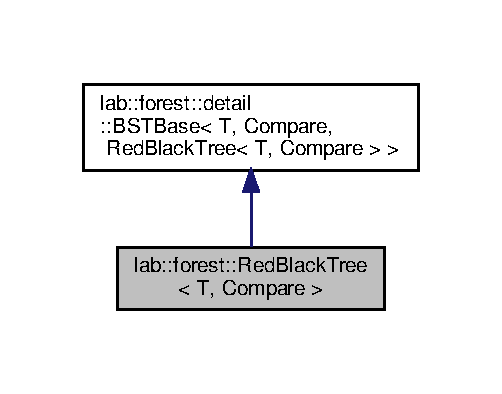
\includegraphics[width=241pt]{classlab_1_1forest_1_1RedBlackTree__inherit__graph}
\end{center}
\end{figure}


Collaboration diagram for lab\+:\+:forest\+:\+:Red\+Black\+Tree$<$ T, Compare $>$\+:
\nopagebreak
\begin{figure}[H]
\begin{center}
\leavevmode
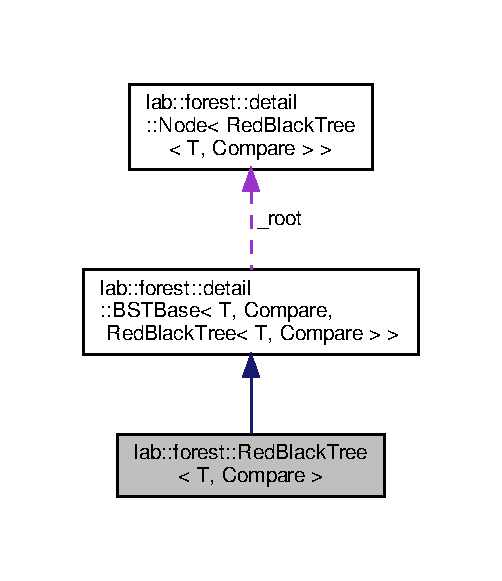
\includegraphics[width=241pt]{classlab_1_1forest_1_1RedBlackTree__coll__graph}
\end{center}
\end{figure}
\subsection*{Public Member Functions}
\begin{DoxyCompactItemize}
\item 
\mbox{\Hypertarget{classlab_1_1forest_1_1RedBlackTree_a50e09d93668a4ad79e2cb90e43fc8136}\label{classlab_1_1forest_1_1RedBlackTree_a50e09d93668a4ad79e2cb90e43fc8136}} 
{\bfseries Red\+Black\+Tree} (const Compare \&comp=Compare \{\})
\item 
\mbox{\Hypertarget{classlab_1_1forest_1_1RedBlackTree_aa067218aae3ec9bdd1be4ece7d6c4ff7}\label{classlab_1_1forest_1_1RedBlackTree_aa067218aae3ec9bdd1be4ece7d6c4ff7}} 
{\footnotesize template$<$typename Iter $>$ }\\\hyperlink{classlab_1_1forest_1_1RedBlackTree_aa067218aae3ec9bdd1be4ece7d6c4ff7}{Red\+Black\+Tree} (Iter \hyperlink{classlab_1_1forest_1_1detail_1_1BSTBase_aee57d4461130971ad187ea41bc8e4e74}{begin}, Iter \hyperlink{classlab_1_1forest_1_1detail_1_1BSTBase_ad2ea364cc61d5581a861d1aab3734129}{end})
\begin{DoxyCompactList}\small\item\em Contructs tree with elements from range \mbox{[}begin, end) \end{DoxyCompactList}\item 
\mbox{\Hypertarget{classlab_1_1forest_1_1RedBlackTree_ac1098111d7495f6640b531344496456b}\label{classlab_1_1forest_1_1RedBlackTree_ac1098111d7495f6640b531344496456b}} 
\hyperlink{classlab_1_1forest_1_1RedBlackTree_ac1098111d7495f6640b531344496456b}{Red\+Black\+Tree} (std\+::initializer\+\_\+list$<$ T $>$ elems)
\begin{DoxyCompactList}\small\item\em Contructs tree with elements from list. \end{DoxyCompactList}\item 
\mbox{\Hypertarget{classlab_1_1forest_1_1RedBlackTree_a80a7256b0b3f65d1592d653754d780c0}\label{classlab_1_1forest_1_1RedBlackTree_a80a7256b0b3f65d1592d653754d780c0}} 
{\bfseries Red\+Black\+Tree} (const \hyperlink{classlab_1_1forest_1_1RedBlackTree}{Red\+Black\+Tree} \&other)=default
\item 
\mbox{\Hypertarget{classlab_1_1forest_1_1RedBlackTree_a4b53ce03c8b61782fcd49e372cbd8b85}\label{classlab_1_1forest_1_1RedBlackTree_a4b53ce03c8b61782fcd49e372cbd8b85}} 
{\bfseries Red\+Black\+Tree} (\hyperlink{classlab_1_1forest_1_1RedBlackTree}{Red\+Black\+Tree} \&\&other) noexcept=default
\item 
\mbox{\Hypertarget{classlab_1_1forest_1_1RedBlackTree_a903afb4432a34d898c818e97a2b18a26}\label{classlab_1_1forest_1_1RedBlackTree_a903afb4432a34d898c818e97a2b18a26}} 
\hyperlink{classlab_1_1forest_1_1RedBlackTree}{Red\+Black\+Tree} \& {\bfseries operator=} (const \hyperlink{classlab_1_1forest_1_1RedBlackTree}{Red\+Black\+Tree} \&other)=default
\item 
\mbox{\Hypertarget{classlab_1_1forest_1_1RedBlackTree_a1f2866ff748b05991b8c4d4501db64ca}\label{classlab_1_1forest_1_1RedBlackTree_a1f2866ff748b05991b8c4d4501db64ca}} 
\hyperlink{classlab_1_1forest_1_1RedBlackTree}{Red\+Black\+Tree} \& {\bfseries operator=} (\hyperlink{classlab_1_1forest_1_1RedBlackTree}{Red\+Black\+Tree} \&\&other) noexcept=default
\end{DoxyCompactItemize}
\subsection*{Friends}
\begin{DoxyCompactItemize}
\item 
\mbox{\Hypertarget{classlab_1_1forest_1_1RedBlackTree_a0366a00ceb99298e94189e0ae094e6d9}\label{classlab_1_1forest_1_1RedBlackTree_a0366a00ceb99298e94189e0ae094e6d9}} 
class {\bfseries detail\+::\+B\+S\+T\+Base$<$ T, Compare, Red\+Black\+Tree$<$ T, Compare $>$ $>$}
\end{DoxyCompactItemize}
\subsection*{Additional Inherited Members}


\subsection{Detailed Description}
\subsubsection*{template$<$typename T, typename Compare = std\+::less$<$$>$$>$\newline
class lab\+::forest\+::\+Red\+Black\+Tree$<$ T, Compare $>$}

Red-\/\+Black Tree implementation T -\/ type of value stored in tree, Compare -\/ comparison function class for elements in tree. 

The documentation for this class was generated from the following file\+:\begin{DoxyCompactItemize}
\item 
include/Red\+Black\+Tree.\+hpp\end{DoxyCompactItemize}

\hypertarget{classlab_1_1forest_1_1SplayTree}{}\section{lab\+:\+:forest\+:\+:Splay\+Tree$<$ T, Compare $>$ Class Template Reference}
\label{classlab_1_1forest_1_1SplayTree}\index{lab\+::forest\+::\+Splay\+Tree$<$ T, Compare $>$@{lab\+::forest\+::\+Splay\+Tree$<$ T, Compare $>$}}


Splay Tree implementation T -\/ type of value stored in tree, Compare -\/ comparison function class for elements in tree.  




{\ttfamily \#include $<$Splay\+Tree.\+hpp$>$}



Inheritance diagram for lab\+:\+:forest\+:\+:Splay\+Tree$<$ T, Compare $>$\+:
\nopagebreak
\begin{figure}[H]
\begin{center}
\leavevmode
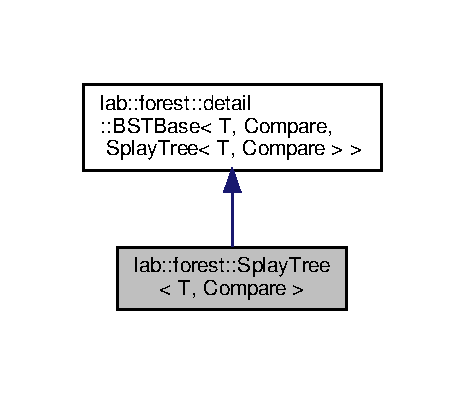
\includegraphics[width=223pt]{classlab_1_1forest_1_1SplayTree__inherit__graph}
\end{center}
\end{figure}


Collaboration diagram for lab\+:\+:forest\+:\+:Splay\+Tree$<$ T, Compare $>$\+:
\nopagebreak
\begin{figure}[H]
\begin{center}
\leavevmode
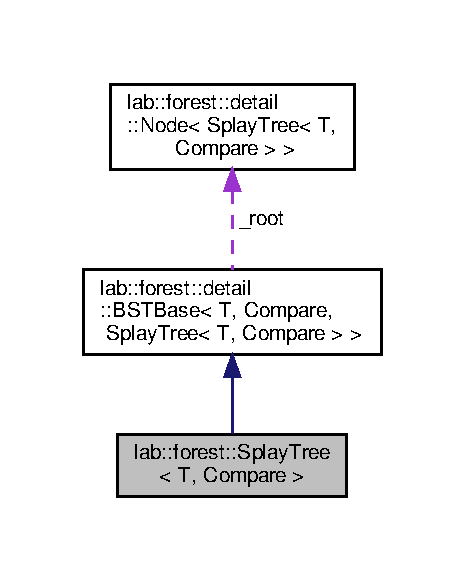
\includegraphics[width=223pt]{classlab_1_1forest_1_1SplayTree__coll__graph}
\end{center}
\end{figure}
\subsection*{Public Member Functions}
\begin{DoxyCompactItemize}
\item 
\mbox{\Hypertarget{classlab_1_1forest_1_1SplayTree_ad174966dcd61b790db0ca1f58e830385}\label{classlab_1_1forest_1_1SplayTree_ad174966dcd61b790db0ca1f58e830385}} 
\hyperlink{classlab_1_1forest_1_1SplayTree_ad174966dcd61b790db0ca1f58e830385}{Splay\+Tree} (const Compare \&comp=Compare\{\}) noexcept
\begin{DoxyCompactList}\small\item\em Creates tree with no elements. \end{DoxyCompactList}\item 
\mbox{\Hypertarget{classlab_1_1forest_1_1SplayTree_aaa4d86c652110bde313d44c614620a83}\label{classlab_1_1forest_1_1SplayTree_aaa4d86c652110bde313d44c614620a83}} 
{\footnotesize template$<$typename Iter $>$ }\\\hyperlink{classlab_1_1forest_1_1SplayTree_aaa4d86c652110bde313d44c614620a83}{Splay\+Tree} (Iter \hyperlink{classlab_1_1forest_1_1detail_1_1BSTBase_aee57d4461130971ad187ea41bc8e4e74}{begin}, Iter \hyperlink{classlab_1_1forest_1_1detail_1_1BSTBase_ad2ea364cc61d5581a861d1aab3734129}{end})
\begin{DoxyCompactList}\small\item\em Contructs tree with elements from range \mbox{[}begin, end) \end{DoxyCompactList}\item 
\mbox{\Hypertarget{classlab_1_1forest_1_1SplayTree_aea9bae39a4f74dbc5b58aa597310e119}\label{classlab_1_1forest_1_1SplayTree_aea9bae39a4f74dbc5b58aa597310e119}} 
{\bfseries Splay\+Tree} (const \hyperlink{classlab_1_1forest_1_1SplayTree}{Splay\+Tree} \&other)=default
\item 
\mbox{\Hypertarget{classlab_1_1forest_1_1SplayTree_a0e734b8ca1882575349e3b415a91d58d}\label{classlab_1_1forest_1_1SplayTree_a0e734b8ca1882575349e3b415a91d58d}} 
{\bfseries Splay\+Tree} (\hyperlink{classlab_1_1forest_1_1SplayTree}{Splay\+Tree} \&\&other) noexcept=default
\item 
\mbox{\Hypertarget{classlab_1_1forest_1_1SplayTree_a94b9c8173af74fa3e16cc64734512c56}\label{classlab_1_1forest_1_1SplayTree_a94b9c8173af74fa3e16cc64734512c56}} 
\hyperlink{classlab_1_1forest_1_1SplayTree}{Splay\+Tree} \& {\bfseries operator=} (const \hyperlink{classlab_1_1forest_1_1SplayTree}{Splay\+Tree} \&other)=default
\item 
\mbox{\Hypertarget{classlab_1_1forest_1_1SplayTree_a0b911d6bb9706deb08073dd32564409f}\label{classlab_1_1forest_1_1SplayTree_a0b911d6bb9706deb08073dd32564409f}} 
\hyperlink{classlab_1_1forest_1_1SplayTree}{Splay\+Tree} \& {\bfseries operator=} (\hyperlink{classlab_1_1forest_1_1SplayTree}{Splay\+Tree} \&\&other) noexcept=default
\item 
\mbox{\Hypertarget{classlab_1_1forest_1_1SplayTree_a31ad5b81f62cd1aae5ef95124859817a}\label{classlab_1_1forest_1_1SplayTree_a31ad5b81f62cd1aae5ef95124859817a}} 
\hyperlink{classlab_1_1forest_1_1SplayTree_a31ad5b81f62cd1aae5ef95124859817a}{Splay\+Tree} (std\+::initializer\+\_\+list$<$ T $>$ elems)
\begin{DoxyCompactList}\small\item\em Contructs tree with elements from list. \end{DoxyCompactList}\end{DoxyCompactItemize}
\subsection*{Friends}
\begin{DoxyCompactItemize}
\item 
\mbox{\Hypertarget{classlab_1_1forest_1_1SplayTree_a48b849668934ff66df6b9e92ced3e9d6}\label{classlab_1_1forest_1_1SplayTree_a48b849668934ff66df6b9e92ced3e9d6}} 
class {\bfseries detail\+::\+B\+S\+T\+Base$<$ T, Compare, Splay\+Tree$<$ T, Compare $>$ $>$}
\end{DoxyCompactItemize}
\subsection*{Additional Inherited Members}


\subsection{Detailed Description}
\subsubsection*{template$<$typename T, typename Compare = std\+::less$<$$>$$>$\newline
class lab\+::forest\+::\+Splay\+Tree$<$ T, Compare $>$}

Splay Tree implementation T -\/ type of value stored in tree, Compare -\/ comparison function class for elements in tree. 

The documentation for this class was generated from the following file\+:\begin{DoxyCompactItemize}
\item 
include/Splay\+Tree.\+hpp\end{DoxyCompactItemize}

\hypertarget{classlab_1_1TreeDatabase}{}\section{lab\+:\+:Tree\+Database Class Reference}
\label{classlab_1_1TreeDatabase}\index{lab\+::\+Tree\+Database@{lab\+::\+Tree\+Database}}


Singleton class represention S\+Q\+Lite-\/based database for tree (can be any container)  




{\ttfamily \#include $<$Tree\+D\+B.\+hpp$>$}

\subsection*{Public Member Functions}
\begin{DoxyCompactItemize}
\item 
\mbox{\Hypertarget{classlab_1_1TreeDatabase_ae95a7773c49745b73e42719762cc2473}\label{classlab_1_1TreeDatabase_ae95a7773c49745b73e42719762cc2473}} 
{\bfseries Tree\+Database} (const \hyperlink{classlab_1_1TreeDatabase}{Tree\+Database} \&other)=delete
\item 
\mbox{\Hypertarget{classlab_1_1TreeDatabase_ad203ea6aff9ad9538599dc6bd49168d1}\label{classlab_1_1TreeDatabase_ad203ea6aff9ad9538599dc6bd49168d1}} 
\hyperlink{classlab_1_1TreeDatabase}{Tree\+Database} \& {\bfseries operator=} (\hyperlink{classlab_1_1TreeDatabase}{Tree\+Database} other)=delete
\item 
\mbox{\Hypertarget{classlab_1_1TreeDatabase_adae6b9244ea8156fe2ca5895839b0a83}\label{classlab_1_1TreeDatabase_adae6b9244ea8156fe2ca5895839b0a83}} 
{\footnotesize template$<$typename Tree $>$ }\\void \hyperlink{classlab_1_1TreeDatabase_adae6b9244ea8156fe2ca5895839b0a83}{save} (const Tree \&\+\_\+tree, std\+::string\+\_\+view name)
\begin{DoxyCompactList}\small\item\em Save tree with name to database. \end{DoxyCompactList}\item 
auto \hyperlink{classlab_1_1TreeDatabase_ad465665c67abac43de6eac1820e1320f}{load\+Names} () -\/$>$ std\+::vector$<$ std\+::string $>$
\item 
{\footnotesize template$<$typename Tree $>$ }\\auto \hyperlink{classlab_1_1TreeDatabase_a9e8daa58f69152466d19cae774c073f1}{load} (std\+::string\+\_\+view name) -\/$>$ std\+::optional$<$ Tree $>$
\item 
\mbox{\Hypertarget{classlab_1_1TreeDatabase_a789018a165caca390c3df533b7ea243b}\label{classlab_1_1TreeDatabase_a789018a165caca390c3df533b7ea243b}} 
void \hyperlink{classlab_1_1TreeDatabase_a789018a165caca390c3df533b7ea243b}{remove} (std\+::string\+\_\+view name)
\begin{DoxyCompactList}\small\item\em Remove tree with name name from database;. \end{DoxyCompactList}\end{DoxyCompactItemize}
\subsection*{Static Public Member Functions}
\begin{DoxyCompactItemize}
\item 
static \hyperlink{classlab_1_1TreeDatabase}{Tree\+Database} \& \hyperlink{classlab_1_1TreeDatabase_a0bc7dc24713be90902d3a58ed66a4d4d}{instance} ()
\end{DoxyCompactItemize}


\subsection{Detailed Description}
Singleton class represention S\+Q\+Lite-\/based database for tree (can be any container) 

Class operating file with database with filename trees.\+sqlite located in output binary directory 

\subsection{Member Function Documentation}
\mbox{\Hypertarget{classlab_1_1TreeDatabase_a0bc7dc24713be90902d3a58ed66a4d4d}\label{classlab_1_1TreeDatabase_a0bc7dc24713be90902d3a58ed66a4d4d}} 
\index{lab\+::\+Tree\+Database@{lab\+::\+Tree\+Database}!instance@{instance}}
\index{instance@{instance}!lab\+::\+Tree\+Database@{lab\+::\+Tree\+Database}}
\subsubsection{\texorpdfstring{instance()}{instance()}}
{\footnotesize\ttfamily static \hyperlink{classlab_1_1TreeDatabase}{Tree\+Database}\& lab\+::\+Tree\+Database\+::instance (\begin{DoxyParamCaption}{ }\end{DoxyParamCaption})\hspace{0.3cm}{\ttfamily [static]}}

\begin{DoxyReturn}{Returns}
Database instance 
\end{DoxyReturn}
\mbox{\Hypertarget{classlab_1_1TreeDatabase_a9e8daa58f69152466d19cae774c073f1}\label{classlab_1_1TreeDatabase_a9e8daa58f69152466d19cae774c073f1}} 
\index{lab\+::\+Tree\+Database@{lab\+::\+Tree\+Database}!load@{load}}
\index{load@{load}!lab\+::\+Tree\+Database@{lab\+::\+Tree\+Database}}
\subsubsection{\texorpdfstring{load()}{load()}}
{\footnotesize\ttfamily template$<$typename Tree $>$ \\
auto lab\+::\+Tree\+Database\+::load (\begin{DoxyParamCaption}\item[{std\+::string\+\_\+view}]{name }\end{DoxyParamCaption}) -\/$>$  std\+::optional$<$ Tree $>$}

\begin{DoxyReturn}{Returns}
Tree with name name and type Tree if success, otherwise -\/ std\+::nullopt 
\end{DoxyReturn}
\mbox{\Hypertarget{classlab_1_1TreeDatabase_ad465665c67abac43de6eac1820e1320f}\label{classlab_1_1TreeDatabase_ad465665c67abac43de6eac1820e1320f}} 
\index{lab\+::\+Tree\+Database@{lab\+::\+Tree\+Database}!load\+Names@{load\+Names}}
\index{load\+Names@{load\+Names}!lab\+::\+Tree\+Database@{lab\+::\+Tree\+Database}}
\subsubsection{\texorpdfstring{load\+Names()}{loadNames()}}
{\footnotesize\ttfamily auto lab\+::\+Tree\+Database\+::load\+Names (\begin{DoxyParamCaption}{ }\end{DoxyParamCaption}) -\/$>$  std\+::vector$<$ std\+::string $>$}

\begin{DoxyReturn}{Returns}
Vector of all trees (theis names) in database 
\end{DoxyReturn}


The documentation for this class was generated from the following file\+:\begin{DoxyCompactItemize}
\item 
include/Tree\+D\+B.\+hpp\end{DoxyCompactItemize}

\hypertarget{classlab_1_1forest_1_1UndoableTree}{}\section{lab\+:\+:forest\+:\+:Undoable\+Tree$<$ Tree $>$ Class Template Reference}
\label{classlab_1_1forest_1_1UndoableTree}\index{lab\+::forest\+::\+Undoable\+Tree$<$ Tree $>$@{lab\+::forest\+::\+Undoable\+Tree$<$ Tree $>$}}


Class that expand Tree functionality by undo and redo operations.  




{\ttfamily \#include $<$Undoable\+Tree.\+hpp$>$}

\subsection*{Public Types}
\begin{DoxyCompactItemize}
\item 
\mbox{\Hypertarget{classlab_1_1forest_1_1UndoableTree_aaf637f922a0a607faf87df1122c16275}\label{classlab_1_1forest_1_1UndoableTree_aaf637f922a0a607faf87df1122c16275}} 
using {\bfseries value\+\_\+type} = typename Tree\+::value\+\_\+type
\item 
\mbox{\Hypertarget{classlab_1_1forest_1_1UndoableTree_ab044c0d5b07e9eb29aae99c7d275de0d}\label{classlab_1_1forest_1_1UndoableTree_ab044c0d5b07e9eb29aae99c7d275de0d}} 
using {\bfseries iterator} = typename Tree\+::iterator
\end{DoxyCompactItemize}
\subsection*{Public Member Functions}
\begin{DoxyCompactItemize}
\item 
\mbox{\Hypertarget{classlab_1_1forest_1_1UndoableTree_ac77c3e18c250430b5e13bd015eff0946}\label{classlab_1_1forest_1_1UndoableTree_ac77c3e18c250430b5e13bd015eff0946}} 
{\bfseries Undoable\+Tree} (std\+::initializer\+\_\+list$<$ value\+\_\+type $>$ elems)
\item 
\mbox{\Hypertarget{classlab_1_1forest_1_1UndoableTree_a2c2edafd4a90b4cc0b12212fb6682287}\label{classlab_1_1forest_1_1UndoableTree_a2c2edafd4a90b4cc0b12212fb6682287}} 
{\bfseries Undoable\+Tree} (const \hyperlink{classlab_1_1forest_1_1UndoableTree}{Undoable\+Tree} \&other)=default
\item 
\mbox{\Hypertarget{classlab_1_1forest_1_1UndoableTree_a6827813d5b65bbd4af5a8dd8ca8d6adc}\label{classlab_1_1forest_1_1UndoableTree_a6827813d5b65bbd4af5a8dd8ca8d6adc}} 
{\bfseries Undoable\+Tree} (\hyperlink{classlab_1_1forest_1_1UndoableTree}{Undoable\+Tree} \&\&other) noexcept=default
\item 
\mbox{\Hypertarget{classlab_1_1forest_1_1UndoableTree_a88123444da2ca4a1068de8d9bf0f04f6}\label{classlab_1_1forest_1_1UndoableTree_a88123444da2ca4a1068de8d9bf0f04f6}} 
\hyperlink{classlab_1_1forest_1_1UndoableTree}{Undoable\+Tree} \& {\bfseries operator=} (const \hyperlink{classlab_1_1forest_1_1UndoableTree}{Undoable\+Tree} \&other)=default
\item 
\mbox{\Hypertarget{classlab_1_1forest_1_1UndoableTree_a38b331baf68b85d65e8bbf85f40f8d95}\label{classlab_1_1forest_1_1UndoableTree_a38b331baf68b85d65e8bbf85f40f8d95}} 
\hyperlink{classlab_1_1forest_1_1UndoableTree}{Undoable\+Tree} \& {\bfseries operator=} (\hyperlink{classlab_1_1forest_1_1UndoableTree}{Undoable\+Tree} \&\&other) noexcept=default
\item 
\mbox{\Hypertarget{classlab_1_1forest_1_1UndoableTree_ab0247c252d8c3ad9fa79c5f2d791a1e3}\label{classlab_1_1forest_1_1UndoableTree_ab0247c252d8c3ad9fa79c5f2d791a1e3}} 
{\footnotesize template$<$typename Iter $>$ }\\{\bfseries Undoable\+Tree} (Iter \hyperlink{classlab_1_1forest_1_1UndoableTree_a70250f012747174b8935cf9fe5fe72ed}{begin}, Iter \hyperlink{classlab_1_1forest_1_1UndoableTree_af404b6bb41ddad0291cf2ab22deee478}{end})
\item 
\mbox{\Hypertarget{classlab_1_1forest_1_1UndoableTree_aed97dba3340b6aec26acac81d23c8525}\label{classlab_1_1forest_1_1UndoableTree_aed97dba3340b6aec26acac81d23c8525}} 
void \hyperlink{classlab_1_1forest_1_1UndoableTree_aed97dba3340b6aec26acac81d23c8525}{insert} (const value\+\_\+type \&key)
\begin{DoxyCompactList}\small\item\em Inserts key to tree. \end{DoxyCompactList}\item 
\mbox{\Hypertarget{classlab_1_1forest_1_1UndoableTree_a5d24d3854ab12114b6d6184ecdd21f56}\label{classlab_1_1forest_1_1UndoableTree_a5d24d3854ab12114b6d6184ecdd21f56}} 
void \hyperlink{classlab_1_1forest_1_1UndoableTree_a5d24d3854ab12114b6d6184ecdd21f56}{erase} (const value\+\_\+type \&key)
\begin{DoxyCompactList}\small\item\em Erase element with this key from tree. \end{DoxyCompactList}\item 
void \hyperlink{classlab_1_1forest_1_1UndoableTree_a4f19003d8156b047de5ff2869d5ac316}{undo} ()
\begin{DoxyCompactList}\small\item\em Undos last done operation (insert or erase) in tree. \end{DoxyCompactList}\item 
\mbox{\Hypertarget{classlab_1_1forest_1_1UndoableTree_a809f804c937c5963f4370ec7312eae0e}\label{classlab_1_1forest_1_1UndoableTree_a809f804c937c5963f4370ec7312eae0e}} 
void \hyperlink{classlab_1_1forest_1_1UndoableTree_a809f804c937c5963f4370ec7312eae0e}{redo} ()
\begin{DoxyCompactList}\small\item\em Redos last undone operation (insert or erase) in tree. \end{DoxyCompactList}\item 
iterator \hyperlink{classlab_1_1forest_1_1UndoableTree_a6e21757708a93c084d55f2b95874d8df}{search} (const value\+\_\+type \&key) noexcept
\item 
\mbox{\Hypertarget{classlab_1_1forest_1_1UndoableTree_a70250f012747174b8935cf9fe5fe72ed}\label{classlab_1_1forest_1_1UndoableTree_a70250f012747174b8935cf9fe5fe72ed}} 
auto \hyperlink{classlab_1_1forest_1_1UndoableTree_a70250f012747174b8935cf9fe5fe72ed}{begin} () const noexcept -\/$>$ iterator
\begin{DoxyCompactList}\small\item\em Inserts key to tree. \end{DoxyCompactList}\item 
\mbox{\Hypertarget{classlab_1_1forest_1_1UndoableTree_af404b6bb41ddad0291cf2ab22deee478}\label{classlab_1_1forest_1_1UndoableTree_af404b6bb41ddad0291cf2ab22deee478}} 
auto \hyperlink{classlab_1_1forest_1_1UndoableTree_af404b6bb41ddad0291cf2ab22deee478}{end} () const noexcept -\/$>$ iterator
\begin{DoxyCompactList}\small\item\em Erase element with this key from tree. \end{DoxyCompactList}\item 
auto \hyperlink{classlab_1_1forest_1_1UndoableTree_a072971d83f1ef40d64f182f0246732ad}{size} () const noexcept -\/$>$ std\+::size\+\_\+t
\item 
auto \hyperlink{classlab_1_1forest_1_1UndoableTree_a359735c6419c5ec92e89f18a29d0a189}{compare\+Func} () const noexcept
\item 
\mbox{\Hypertarget{classlab_1_1forest_1_1UndoableTree_a35bf2be1b8f96375aee133feef6447b9}\label{classlab_1_1forest_1_1UndoableTree_a35bf2be1b8f96375aee133feef6447b9}} 
bool {\bfseries operator==} (const \hyperlink{classlab_1_1forest_1_1UndoableTree}{Undoable\+Tree} \&other) const noexcept
\item 
\mbox{\Hypertarget{classlab_1_1forest_1_1UndoableTree_aaf614d1b26cca3a935adaf7badb2a493}\label{classlab_1_1forest_1_1UndoableTree_aaf614d1b26cca3a935adaf7badb2a493}} 
bool {\bfseries operator!=} (const \hyperlink{classlab_1_1forest_1_1UndoableTree}{Undoable\+Tree} \&other) const noexcept
\end{DoxyCompactItemize}


\subsection{Detailed Description}
\subsubsection*{template$<$typename Tree$>$\newline
class lab\+::forest\+::\+Undoable\+Tree$<$ Tree $>$}

Class that expand Tree functionality by undo and redo operations. 

\subsection{Member Function Documentation}
\mbox{\Hypertarget{classlab_1_1forest_1_1UndoableTree_a359735c6419c5ec92e89f18a29d0a189}\label{classlab_1_1forest_1_1UndoableTree_a359735c6419c5ec92e89f18a29d0a189}} 
\index{lab\+::forest\+::\+Undoable\+Tree@{lab\+::forest\+::\+Undoable\+Tree}!compare\+Func@{compare\+Func}}
\index{compare\+Func@{compare\+Func}!lab\+::forest\+::\+Undoable\+Tree@{lab\+::forest\+::\+Undoable\+Tree}}
\subsubsection{\texorpdfstring{compare\+Func()}{compareFunc()}}
{\footnotesize\ttfamily template$<$typename Tree $>$ \\
auto \hyperlink{classlab_1_1forest_1_1UndoableTree}{lab\+::forest\+::\+Undoable\+Tree}$<$ Tree $>$\+::compare\+Func (\begin{DoxyParamCaption}{ }\end{DoxyParamCaption}) const\hspace{0.3cm}{\ttfamily [noexcept]}}

\begin{DoxyReturn}{Returns}
Function that sets order in tree, default -\/ std\+::less\{\} 
\end{DoxyReturn}
\mbox{\Hypertarget{classlab_1_1forest_1_1UndoableTree_a6e21757708a93c084d55f2b95874d8df}\label{classlab_1_1forest_1_1UndoableTree_a6e21757708a93c084d55f2b95874d8df}} 
\index{lab\+::forest\+::\+Undoable\+Tree@{lab\+::forest\+::\+Undoable\+Tree}!search@{search}}
\index{search@{search}!lab\+::forest\+::\+Undoable\+Tree@{lab\+::forest\+::\+Undoable\+Tree}}
\subsubsection{\texorpdfstring{search()}{search()}}
{\footnotesize\ttfamily template$<$typename Tree $>$ \\
iterator \hyperlink{classlab_1_1forest_1_1UndoableTree}{lab\+::forest\+::\+Undoable\+Tree}$<$ Tree $>$\+::search (\begin{DoxyParamCaption}\item[{const value\+\_\+type \&}]{key }\end{DoxyParamCaption})\hspace{0.3cm}{\ttfamily [noexcept]}}

\begin{DoxyReturn}{Returns}
Iterator to key in tree, if not found -\/ \hyperlink{classlab_1_1forest_1_1UndoableTree_af404b6bb41ddad0291cf2ab22deee478}{end()} 
\end{DoxyReturn}
\mbox{\Hypertarget{classlab_1_1forest_1_1UndoableTree_a072971d83f1ef40d64f182f0246732ad}\label{classlab_1_1forest_1_1UndoableTree_a072971d83f1ef40d64f182f0246732ad}} 
\index{lab\+::forest\+::\+Undoable\+Tree@{lab\+::forest\+::\+Undoable\+Tree}!size@{size}}
\index{size@{size}!lab\+::forest\+::\+Undoable\+Tree@{lab\+::forest\+::\+Undoable\+Tree}}
\subsubsection{\texorpdfstring{size()}{size()}}
{\footnotesize\ttfamily template$<$typename Tree $>$ \\
auto \hyperlink{classlab_1_1forest_1_1UndoableTree}{lab\+::forest\+::\+Undoable\+Tree}$<$ Tree $>$\+::size (\begin{DoxyParamCaption}{ }\end{DoxyParamCaption}) const -\/$>$  std\+::size\+\_\+t\hspace{0.3cm}{\ttfamily [noexcept]}}

\begin{DoxyReturn}{Returns}
Amount of elements in tree 
\end{DoxyReturn}
\mbox{\Hypertarget{classlab_1_1forest_1_1UndoableTree_a4f19003d8156b047de5ff2869d5ac316}\label{classlab_1_1forest_1_1UndoableTree_a4f19003d8156b047de5ff2869d5ac316}} 
\index{lab\+::forest\+::\+Undoable\+Tree@{lab\+::forest\+::\+Undoable\+Tree}!undo@{undo}}
\index{undo@{undo}!lab\+::forest\+::\+Undoable\+Tree@{lab\+::forest\+::\+Undoable\+Tree}}
\subsubsection{\texorpdfstring{undo()}{undo()}}
{\footnotesize\ttfamily template$<$typename Tree $>$ \\
void \hyperlink{classlab_1_1forest_1_1UndoableTree}{lab\+::forest\+::\+Undoable\+Tree}$<$ Tree $>$\+::undo (\begin{DoxyParamCaption}{ }\end{DoxyParamCaption})}



Undos last done operation (insert or erase) in tree. 

\begin{DoxyAttention}{Attention}
To undo undo operation -\/ use redo 
\end{DoxyAttention}


The documentation for this class was generated from the following file\+:\begin{DoxyCompactItemize}
\item 
include/Undoable\+Tree.\+hpp\end{DoxyCompactItemize}

%--- End generated contents ---

% Index
\backmatter
\newpage
\phantomsection
\clearemptydoublepage
\addcontentsline{toc}{chapter}{Index}
\printindex

\end{document}
